\documentclass[fontsize=11pt]{jlreq}
\usepackage{subfiles}
\usepackage{amsmath, amssymb, braket} % AMS math
\usepackage{lmodern} % Font for math
\usepackage{graphicx,color} % https://texwiki.texjp.org/?hyperref
\usepackage{subcaption} % Captions for figures, etc.
\usepackage{bm} % bold math
\usepackage{quantikz} % Quantum circuit diagrams
\usepackage[version=4]{mhchem} % Chemical formulas
\usepackage[backend=biber, style=numeric, maxnames=5, doi=false, url=true, eprint=true]{biblatex}
\addbibresource{quantum.bib}
\makeatletter
\let\mkbibemph=\mkbibitalic
\let\blx@imc@mkbibemph=\blx@imc@mkbibitalic
\makeatother
\setlength{\biblabelsep}{0.5em}

%\usepackage{pdfx}  % side-effect: hyperref is also configured
\usepackage{hyperref} % Embed links, generate pdf table of contents
\hypersetup{
    colorlinks=true,
    linkcolor=blue,
    urlcolor=cyan,
    pdftitle={Quantum Circuit for First Quantization Hamiltonian Simulation Handling Coulomb Potential Pole},
    pdfauthor={Hideo Takahashi},
    pdfsubject={Research Paper},
    pdfkeywords={Quantum Computer, First Quantization, ab initio, Simulator, Coulomb Potential, Quantum Chemistry},
    bookmarksnumbered=true,
    bookmarksopen=true
}
\usepackage{paper2025}

\begin{document}
\title{Time Evolution Simulation and Error Analysis of 1D and 2D Hydrogen Atom Models Using Full Quantum Circuits\\
Supplementary Material}
\section{Details on the Method for Determining Simulation Parameters to Minimize Error}
\label{smsec:parameter-selection-for-minimum-error-analysis-details}

Error evaluation when time evolution is performed over a long period.
\begin{figure}[ht]
    \centering
    \begin{subfigure}{0.45\columnwidth}
        \centering
        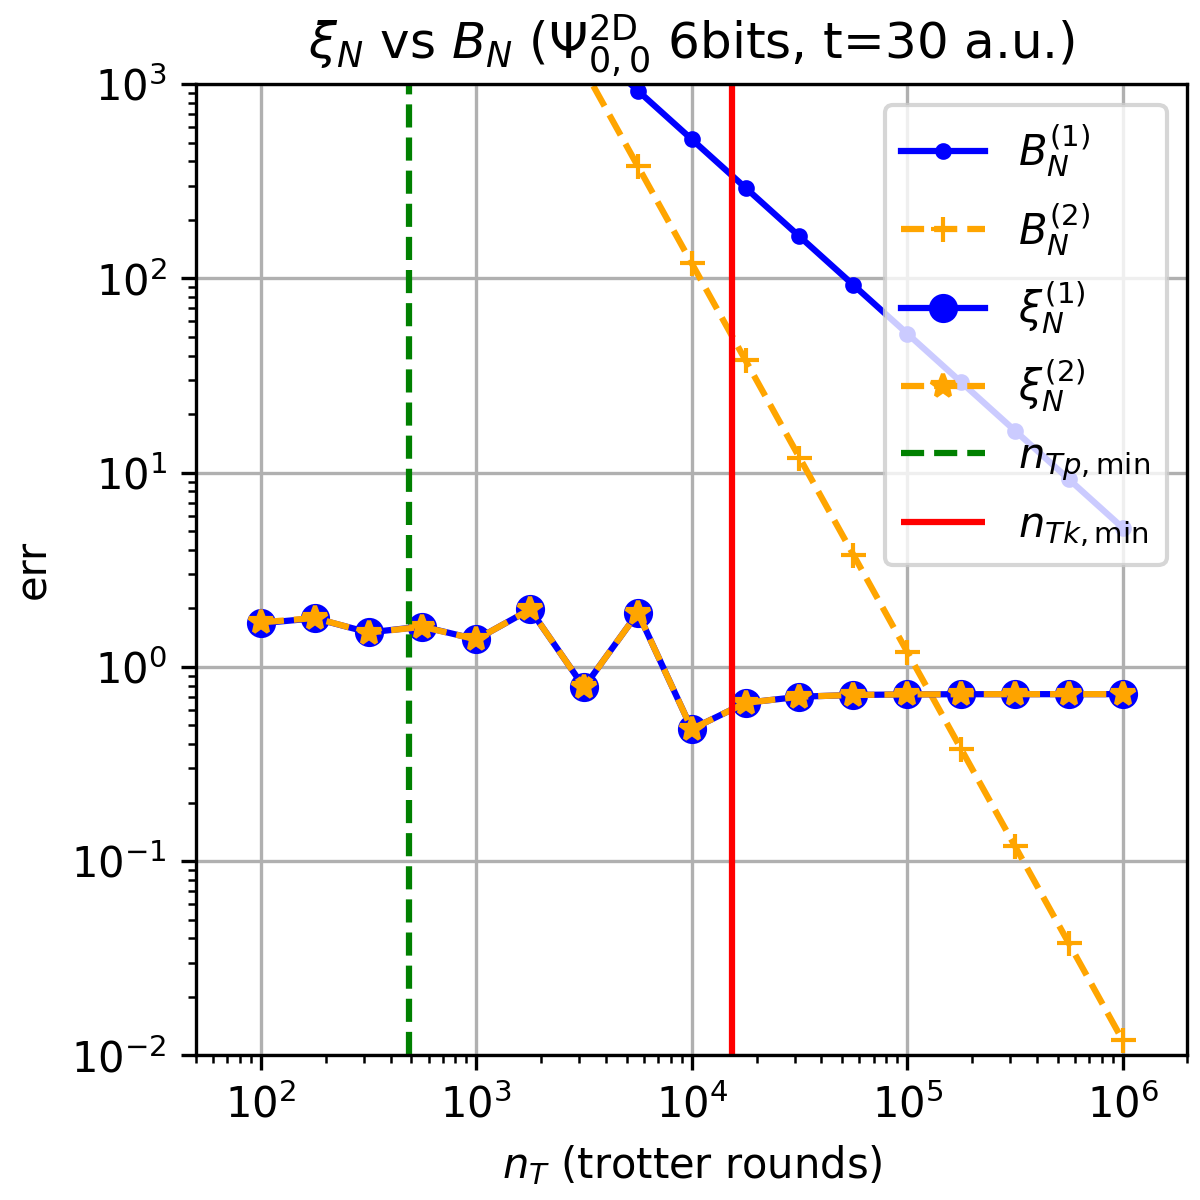
\includegraphics[width=1\columnwidth]{paper2025_figs/sdt_error/trotter_err_n0_m0_6b_t30.png}
        \caption{$\PsiTwoD_{0,0}, \nb=6, t=30.0$}
        \label{subfig:trotter-error-2d-0-0-6b-t30}
    \end{subfigure}
    \begin{subfigure}{0.45\columnwidth}
        \centering
        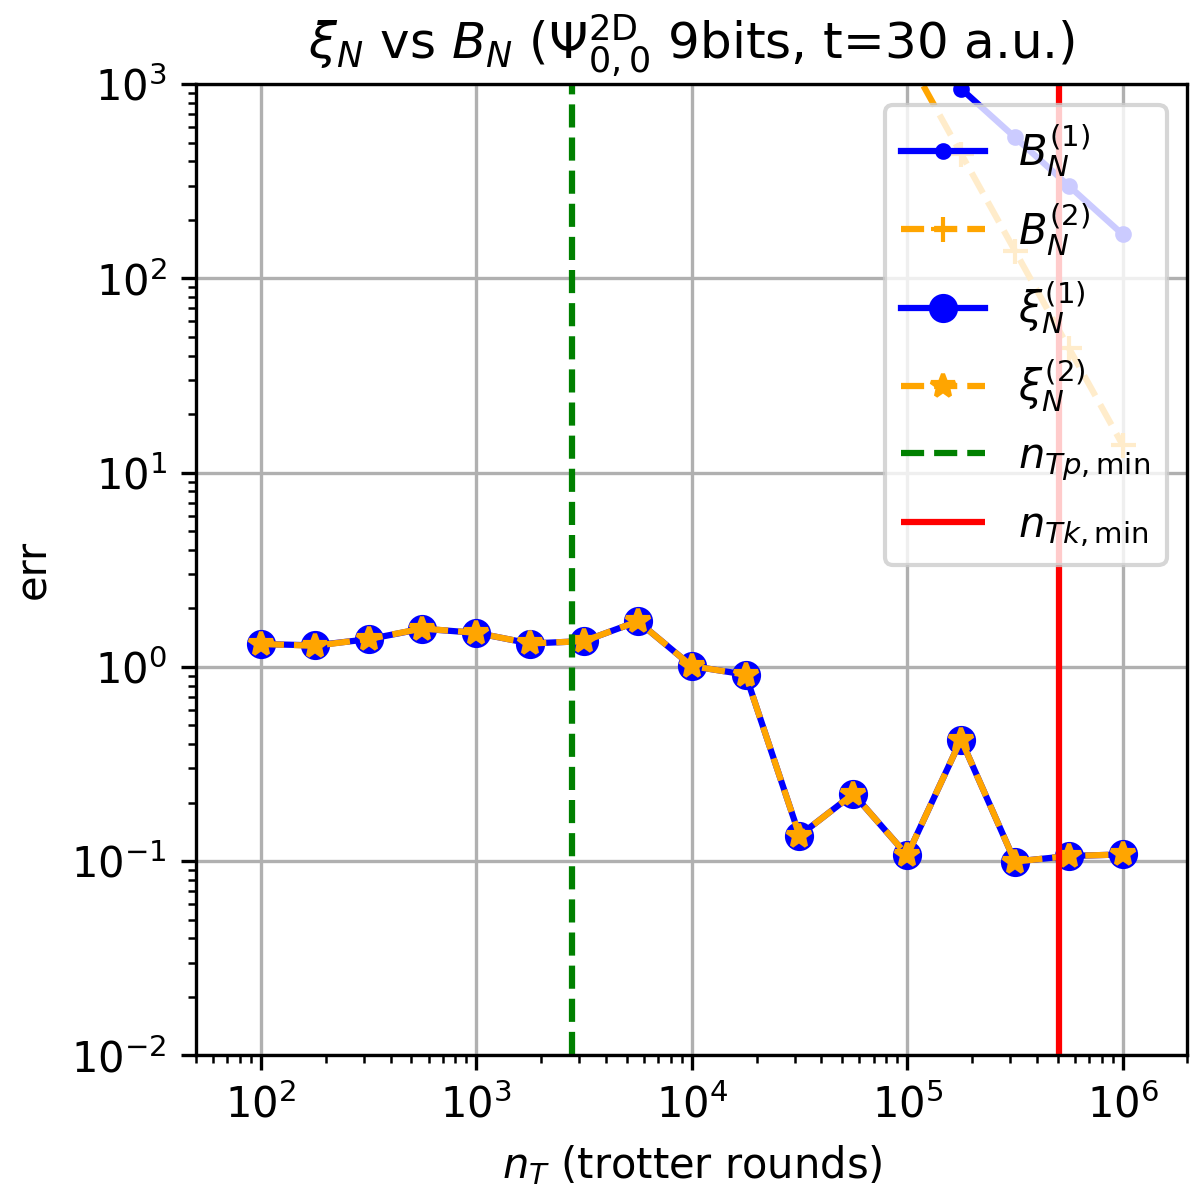
\includegraphics[width=1\columnwidth]{paper2025_figs/sdt_error/trotter_err_n0_m0_9b_t30.png}
        \caption{$\PsiTwoD_{0,0}, \nb=9, t=30.0$}
        \label{subfig:trotter-error-2d-0-0-9b-t30}
    \end{subfigure}

    \begin{subfigure}{0.45\columnwidth}
        \centering
        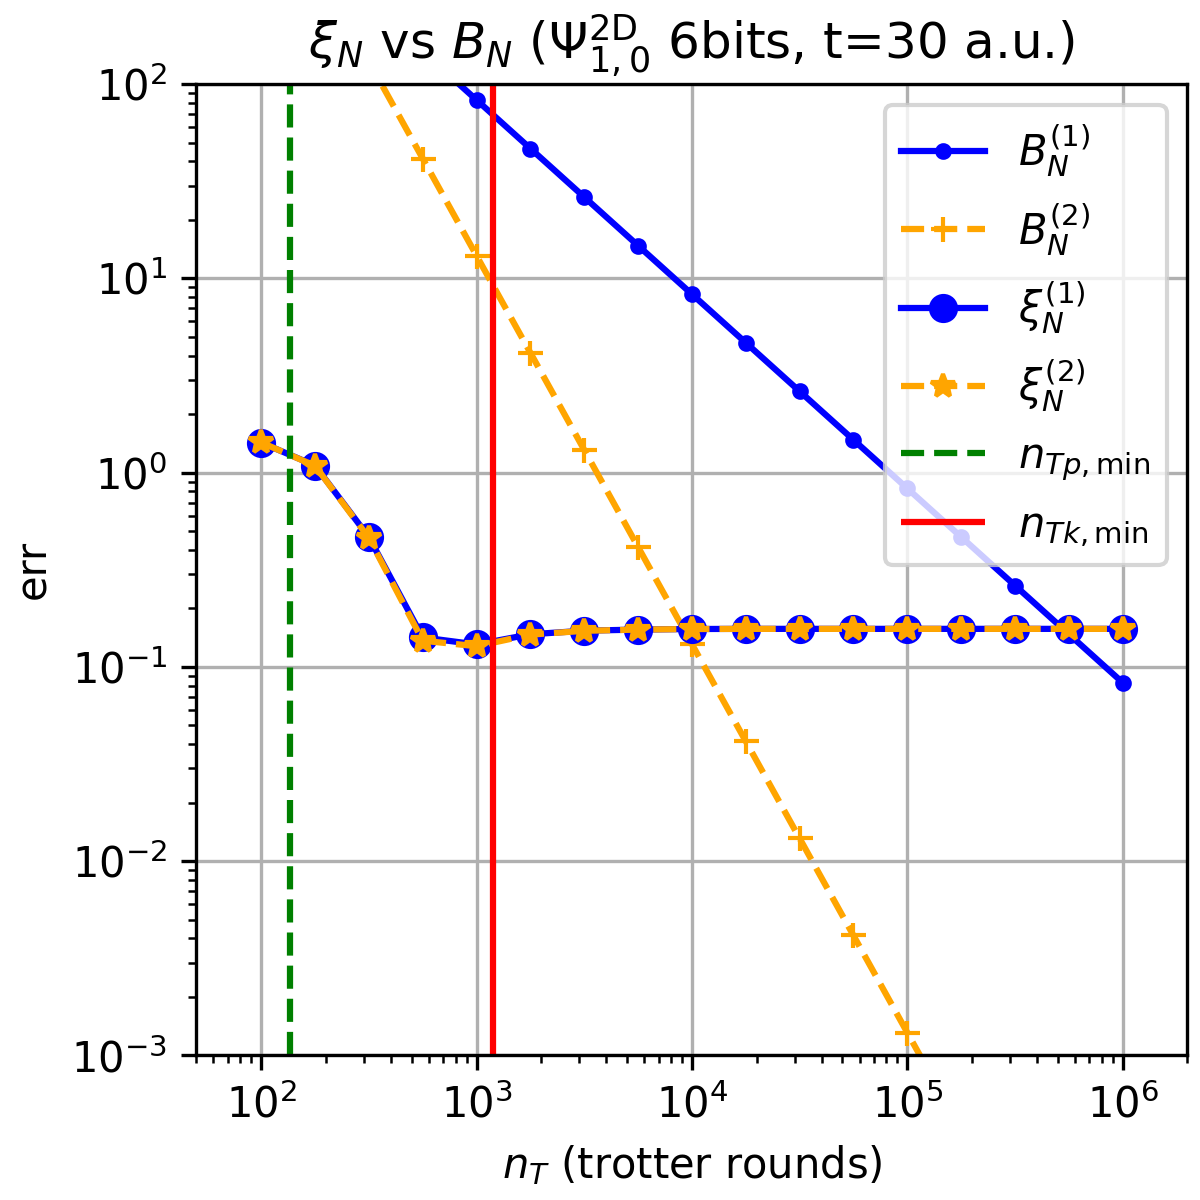
\includegraphics[width=1\columnwidth]{paper2025_figs/sdt_error/trotter_err_n1_m0_6b_t30.png}
        \caption{$\PsiTwoD_{1,0}, \nb=6, t=30.0$}
        \label{subfig:trotter-error-2d-1-0-6b-t30}
    \end{subfigure}
    \begin{subfigure}{0.45\columnwidth}
        \centering
        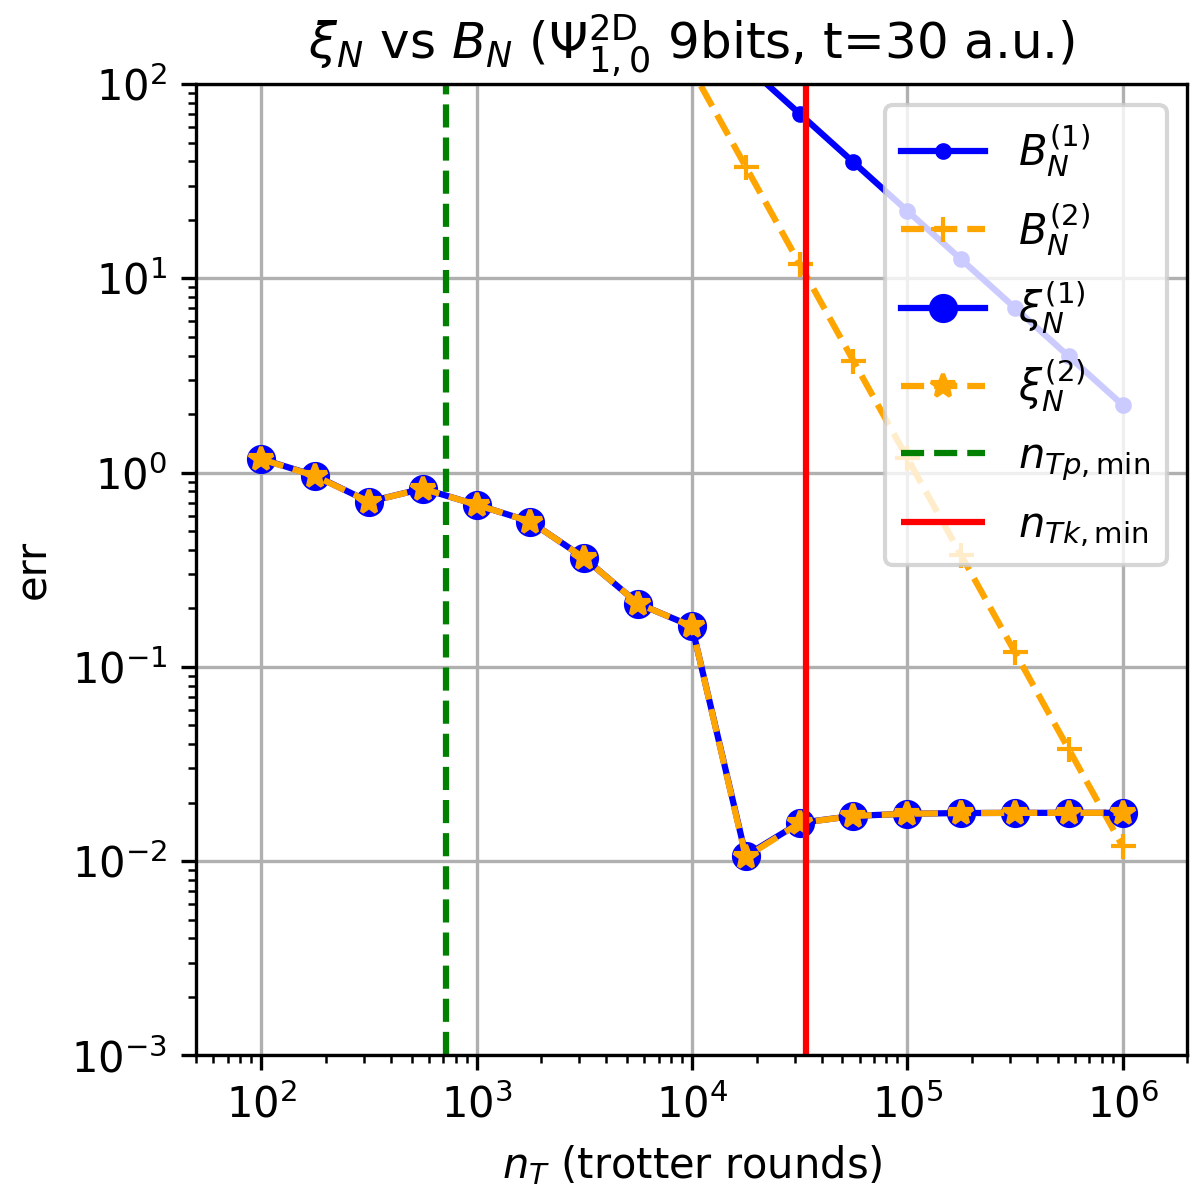
\includegraphics[width=1\columnwidth]{paper2025_figs/sdt_error/trotter_err_n1_m0_9b_t30.png}
        \caption{$\PsiTwoD_{1,0}, \nb=9, t=30.0$}
        \label{subfig:trotter-error-2d-1-0-9b-t30}
    \end{subfigure}

    \caption{Upper bound $\BN{\gamma}$ and observed value $\xiN{\gamma}$ of the error with respect to the number of divisions $\nT$ at time evolution period $t=30.0$}
    \label{fig:trotter-error-t30-part1}
\end{figure}

\begin{figure}[ht]
    \centering
    \begin{subfigure}{0.45\columnwidth}
        \centering
        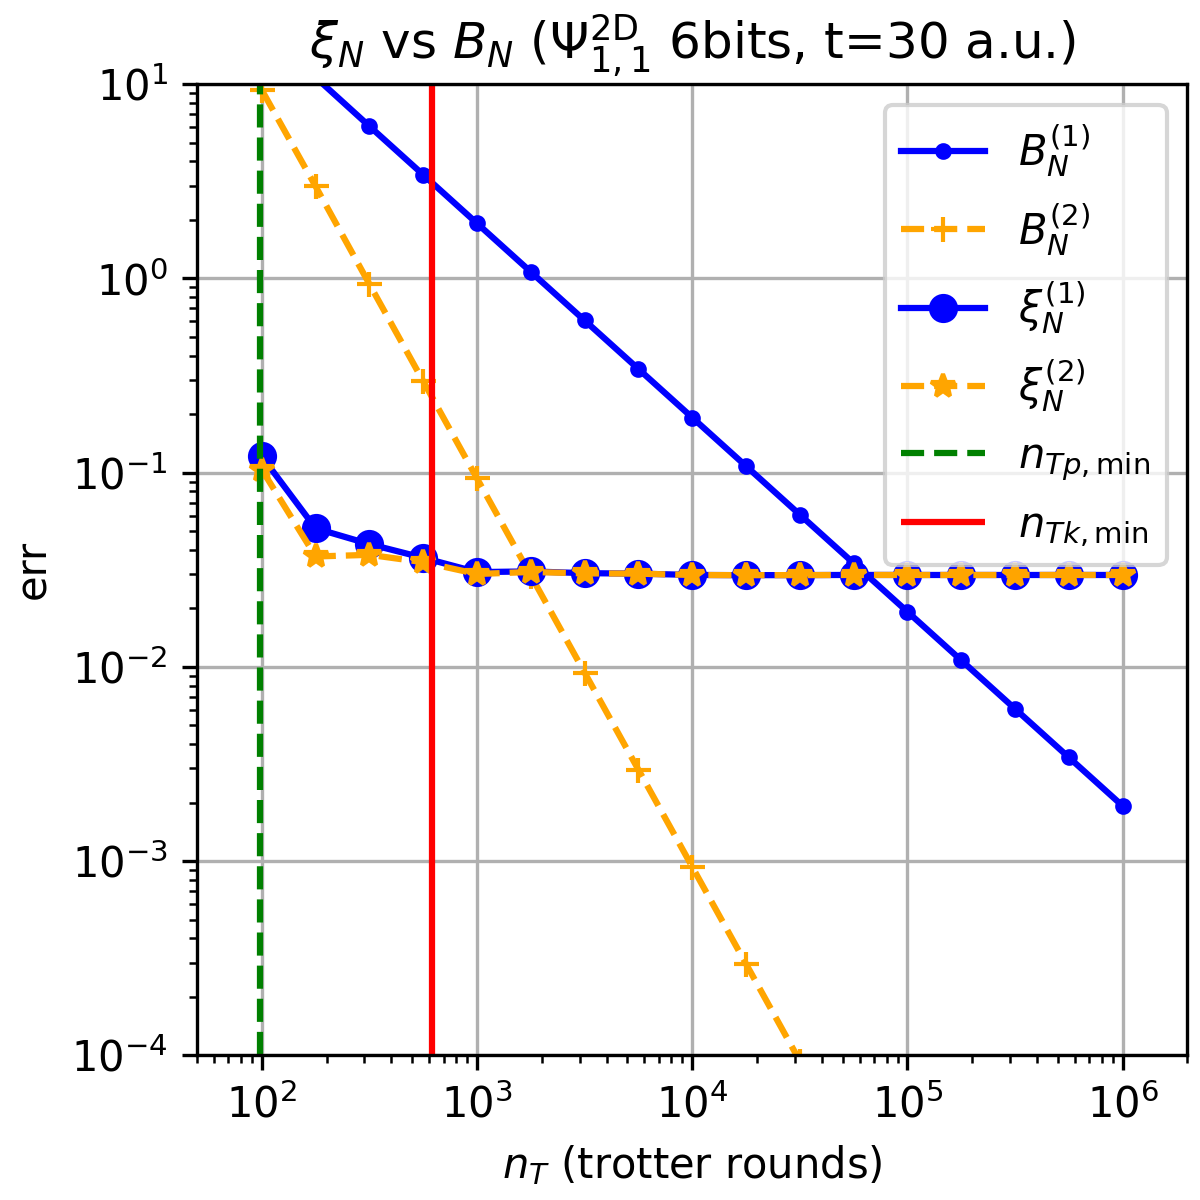
\includegraphics[width=1\columnwidth]{paper2025_figs/sdt_error/trotter_err_n1_m1_6b_t30.png}
        \caption{$\PsiTwoD_{1,1}, \nb=6, t=30.0$}
        \label{subfig:trotter-error-2d-1-1-6b-t30}
    \end{subfigure}
    \begin{subfigure}{0.45\columnwidth}
        \centering
        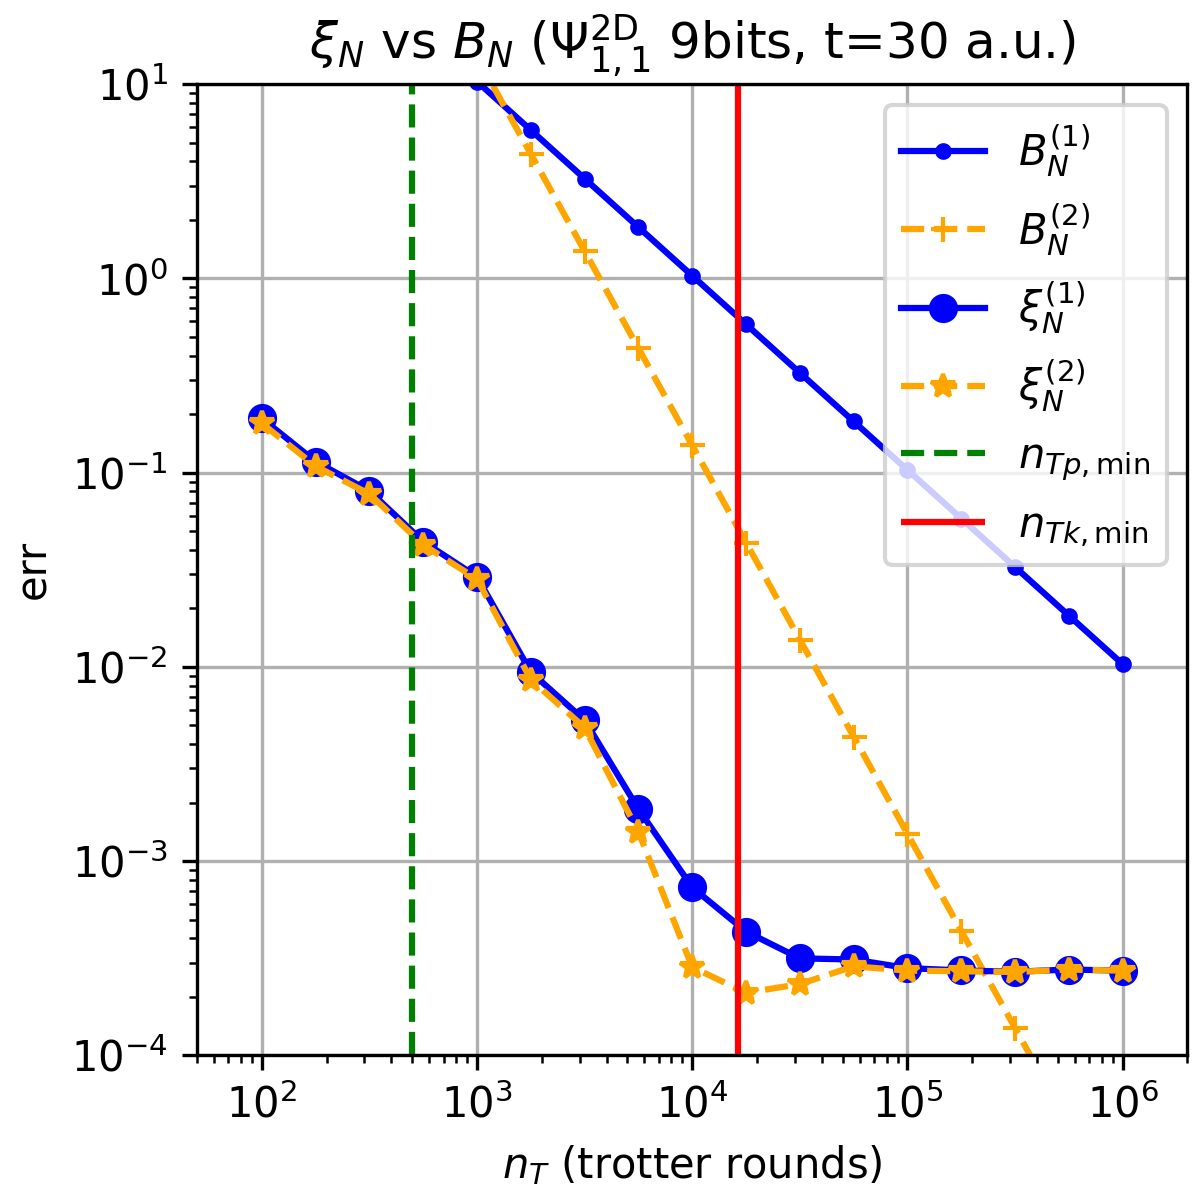
\includegraphics[width=1\columnwidth]{paper2025_figs/sdt_error/trotter_err_n1_m1_9b_t30.png}
        \caption{$\PsiTwoD_{1,1}, \nb=9, t=30.0$}  
        \label{subfig:trotter-error-2d-1-1-9b-t30}
    \end{subfigure}

    \caption{Upper bound $\BN{\gamma}$ and observed value $\xiN{\gamma}$ of the error with respect to the number of divisions $\nT$ at time evolution period $t=30.0$ (continued)}
    \label{fig:trotter-error-t30-part2}
\end{figure}

\end{document}